
\section{FPGA Design Flow and Toolchain}
\label{sec:fpga_flow_toolchain}

Modern FPGA designs require a sophisticated toolchain to bridge the gap between high-level hardware descriptions and the final bitstream used to configure the FPGA. 
Figure~\ref{fig:design_flow} illustrates a representative process that converts an abstract Hardware Description Language (HDL) design into a verified configuration file for a target device.

{
    \centering
    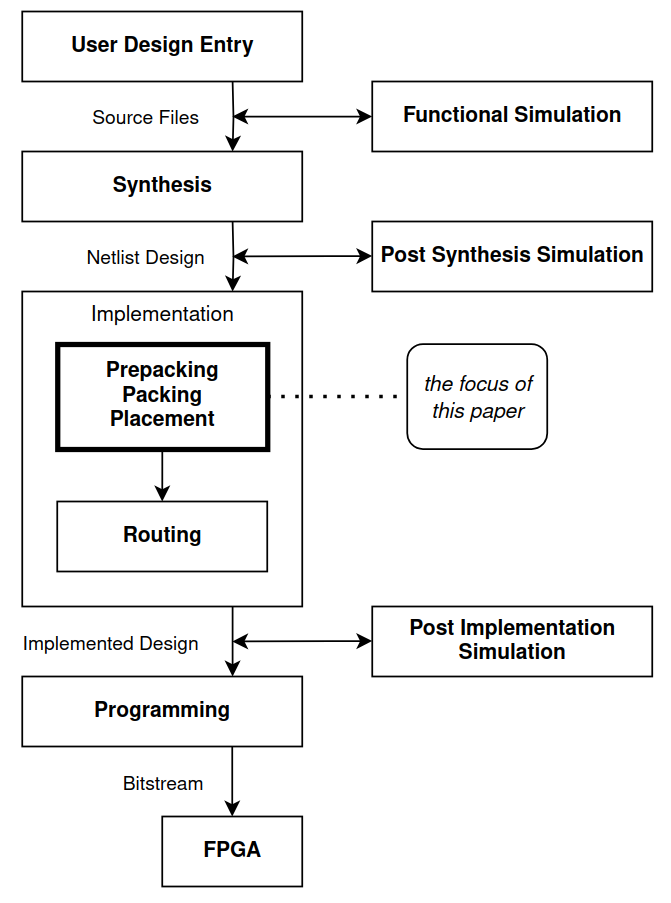
\includegraphics[width=0.9\columnwidth]{figures/design_flow.png}
    \captionof{figure}{A typical FPGA design and verification workflow.}
    \label{fig:design_flow}
}

\begin{enumerate}
\item \textbf{Design Entry:} 
    An engineer describes the intended functionality of the digital system using a hardware description language (HDL) such as Verilog or VHDL. 
    During this phase, the coding style can vary (behavioral, structural, dataflow, etc.), but it generally aims to capture high-level behavior rather than device-specific details.

\item \textbf{Synthesis:} 
    The synthesis tool parses the HDL source, performs logical optimizations, and maps the design onto primitive cells that suit the target FPGA technology. 
    The output is typically a structural \texttt{netlist} (e.g., EDIF or structural Verilog) which details how the design’s logic is broken down into LUTs, FFs, and other vendor-specific cells.

\item \textbf{Placement and Routing (Implementation):} 
    In \emph{placement}, each logical cell from the synthesized netlist is assigned to a physical location on the FPGA fabric. 
    For instance, LUTs and FFs go into specific \emph{BELs} within the device’s CLB sites, and specialized cells such as DSPs and Block RAMs must be placed in their corresponding tile types. 
    Next, \emph{routing} determines how signals are physically wired through the FPGA’s configurable interconnect network. 
    Modern tools often interleave these steps (e.g., fluid-placement routing or routing-aware placement) to better meet timing and area objectives.

\item \textbf{Bitstream Generation:} 
    After a design is fully placed, routed, and timing-closed, the toolchain produces a final \emph{bitstream} that sets the configuration of every programmable element in the FPGA. 
    This bitstream can then be loaded onto the device, either through vendor software or via a custom programming interface.

\item \textbf{Verification:} 
    In parallel to the design flow, simulations and testbenches validate correctness of the user's design at multiple abstraction levels. 
    Engineers may begin with behavioral simulations, then progress to post-synthesis simulations, and finally to post-implementation simulations that incorporate estimated routing delays. 
    With each higher level of fidelity, computational requirements grow significantly due to increasing complexity and the need to analyze more variables over time. 
    Ensuring correct functionality and meeting timing closure at the post-implementation stage is crucial before deploying the design to hardware. 
    Given the importance of thorough verification, many established companies dedicate one verification engineer for every design engineer.
\end{enumerate}

% This workflow underscores the critical role of \textbf{placement} in bridging the netlist to a physical realization. 
% An efficient placement algorithm can drastically reduce compile times and improve design performance, enabling broader adoption of FPGAs in application spaces that require fast design iteration.
